\chapter[Les outils numériques du CMBV]{Les outils numériques du CMBV : historique et écosystème} \label{chap2}

L'histoire des outils numériques du \gls{cmbv} commence au début des années 1990, à une époque où l'informatique documentaire en était encore à ses balbutiements. Le projet \textit{Philidor} naît d'une intuition simple : rassembler dans un même outil l'ensemble des informations relatives au patrimoine musical baroque français. Mais cette ambition initiale va se heurter aux réalités techniques, aux évolutions technologiques et aux besoins croissants des utilisateurs.

Ce chapitre retrace cette histoire mouvementée, faite d'adaptations successives et de migrations plus ou moins complexes. Il montre comment chaque étape technique correspond à des choix stratégiques et révèle des conceptions différentes de ce que doit être un outil patrimonial. De la base JLB-DOC des années 1990 aux solutions contemporaines sous Omeka-S, en passant par les migrations vers \textit{eZ Publish} puis vers des architectures plus spécialisées, cette chronologie technique éclaire les enjeux contemporains.

L'analyse ne se limite pas à une succession d'outils isolés. Elle examine l'écosystème global qui s'est progressivement constitué au \gls{cmbv} : diversification des solutions, spécialisation des usages, interconnexion des données. Cette approche systémique révèle la complexité croissante de l'environnement numérique institutionnel et les défis de cohérence qu'elle engendre.

\section{Les bases de données sous JLB}

Les premiers développements numériques du \gls{cmbv} s'inscrivent dans le paysage technologique des années 1990, dominé par des solutions documentaires propriétaires et des interfaces peu ergonomiques. Cette section retrace la genèse du projet \textit{Philidor}, depuis sa création, simple inventaire informatisé des fonds du centre, jusqu'aux premières tentatives de mise en ligne avec JLB-DOC (\textit{Philidor I}) puis la migration vers JLB-NET (\textit{Philidor II}). Elle analyse les choix techniques de l'époque, contraints par les limitations des technologies disponibles, et montre comment ces premiers développements posent déjà les questions fondamentales qui traverseront toute l'histoire ultérieure de l'outil : structuration des données, ergonomie des interfaces, articulation entre différents types d'informations.

\subsection{Création de la base \textit{Philidor}}

La base de données \textit{Philidor} a été créée en 1990 par Jean Duron, qui restera son responsable scientifique jusqu'en 2007. Cette première version, que l'on peut qualifier de \textit{Philidor} ou \textit{Philidor 0}, constitue le fondement de tous les développements ultérieurs et mérite une analyse détaillée de ses objectifs, de sa structure et de ses modalités de fonctionnement.

\subsubsection{Objectifs fondateurs de la base \textit{Philidor}}

L'objectif principal était de pallier à l'éparpillement des connaissances sur les œuvres musicales. La base a été conçue comme un outil centralisateur permettant de rassembler sur une même notice l'ensemble des informations concernant une œuvre, un musicien ou un événement donné\footcite[Présentation de la base de données PHILIDOR en Février 2004]{michelbenoitDocumentationTechniqueBibliographique1997}. Cette vision unificatrice répondait à un besoin urgent de la communauté scientifique : disposer d'un référentiel commun pour la recherche sur la musique baroque française.

Initialement, \textit{Philidor} était conçu comme une \textquote{aide à l'écriture}, c'est-à-dire comme un outil pour les chercheurs, encadrés par le personnel du \gls{cmbv}, pour réaliser leurs catalogues et bibliographies, ou tout autre projet nécessitant une base de données modulable. Dans un premier temps, la diffusion en ligne n'était pas l'objectif ; les données n'étaient consultables que sur rendez-vous au \glslink{cmbv}{Centre}\footcite[Présentation de la base de données PHILIDOR en Octobre 2010]{michelbenoitDocumentationTechniqueBibliographique1997}. Cette approche \textquote{fermée} correspondait aux pratiques de l'époque, où les bases de données étaient principalement conçues comme des outils internes de travail.

Le système fonctionnait avec le logiciel documentaire JLB-DOC, et les premières années furent consacrées à la saisie massive d'informations à partir de sources originales et de références bibliographiques\footcite[Présentation de la base de données PHILIDOR en Octobre 2010]{michelbenoitDocumentationTechniqueBibliographique1997}. Cette phase de constitution du corpus a nécessité un travail considérable de dépouillement et de normalisation des données.

\subsubsection{Structure et organisation : les différents fichiers composant la base}

En 1997, une réorganisation importante intervint : la base fut scindée en quatre ensembles indépendants, correspondant à des types de données bien distincts. Cette structuration modulaire témoigne d'une approche pragmatique, adaptée aux différents usages et publics visés.

\paragraph{Le fichier \textit{ŒUVRES}} regroupait les notices décrivant des œuvres musicales, théoriques, chorégraphiques ou poétiques du répertoire français des XVII\textsuperscript{e} et XVIII\textsuperscript{e} siècles. Il permettait des recherches par auteur, titre, \gls{incipitmusical} ou textuel, genre, effectif ou dédicataire et a intégré diverses bases de données indépendantes\footcite[Conseil scientifique d'octobre 1997]{michelbenoitDocumentationTechniqueBibliographique1997}. Ce fichier constituait le cœur scientifique de la base, rassemblant l'information musicologique de référence.

\paragraph{Le fichier \textit{BIBLIO}} rassemblait des notices bibliographiques d'ouvrages, de thèses, d'articles et de contributions, publiés à partir de 1800, mais portant sur la musique baroque française. Il permettait des recherches détaillées par mots-clés, lieux, œuvres ou noms de personnes\footcite[Conseil scientifique d'octobre 1997]{michelbenoitDocumentationTechniqueBibliographique1997}. En 1999, il contenait 10 000 notices\footcite[Conseil scientifique de février 1999]{michelbenoitDocumentationTechniqueBibliographique1997}, témoignant de l'ampleur du travail bibliographique accompli.

\paragraph{Le fichier \textit{ARCHIVES}} recensait les documents originaux conservés dans des fonds d'archives comme des actes, des notices de dictionnaires ou des correspondances, en lien avec des personnalités de la vie musicale, administrative ou artistique de l'époque\footcite[Conseil scientifique d'octobre 1997]{michelbenoitDocumentationTechniqueBibliographique1997}. Ce fichier révèle la dimension patrimoniale du projet, qui ne se limitait pas aux œuvres mais embrassait l'ensemble du contexte historique.

\paragraph{Le fichier \textit{ANNUAIRE}} contenait des notices internes sur des spécialistes, des institutions et des lieux, destinées à un usage purement interne au \gls{cmbv}. Il n'était consultable que par le personnel du \glslink{cmbv}{Centre} et servait aussi à l'édition d'étiquettes ou d'un annuaire papier\footcite[Conseil scientifique d'octobre 1997]{michelbenoitDocumentationTechniqueBibliographique1997}. Cette dimension \textquote{carnet d'adresses} illustre la vocation fédératrice du \gls{cmbv} au sein de la communauté scientifique.

\subsubsection{Pratiques de saisie et premiers tests d'interrogation}

Les travaux entrepris à cette période incluaient la normalisation des grilles de saisie pour tous les types de documents, la construction d'un \gls{thesaurus} hiérarchisé permettant une indexation fine et cohérente, ainsi que l'intégration de bases jusque-là indépendantes. Des sessions de formation étaient organisées pour harmoniser les pratiques de saisie entre les différents collaborateurs\footcite[Conseil scientifique d'octobre 1997]{michelbenoitDocumentationTechniqueBibliographique1997}. Cette préoccupation de normalisation témoigne d'une approche professionnelle, soucieuse de la qualité et de la cohérence des données.

En 1997, un test d'interrogation de la base fut réalisé afin d'en évaluer les performances et la pertinence pour la recherche musicologique\footcite[Conseil scientifique d'octobre 1997]{michelbenoitDocumentationTechniqueBibliographique1997}. Si la richesse et la précision des données furent reconnues, il apparut que l'interface d'interrogation était complexe pour un utilisateur non formé, et que la consultation par un public élargi nécessiterait des adaptations. Ce constat préfigure les enjeux d'ergonomie et d'\gls{accessibilite} qui marqueront toute l'évolution ultérieure de l'outil.

\subsection{Une première mise en ligne sous JLB-DOC : \textit{Philidor I}}

La transition vers la mise en ligne marque un tournant conceptuel majeur dans l'histoire de \textit{Philidor}. D'outil interne de travail, la base devient progressivement un service à la disposition du public afin de diffuser les connaissances, avec tous les défis techniques et éditoriaux que cela implique.

\subsubsection{Prémices et stratégie de déploiement}

Sur la fin des années 90, la mise en ligne était envisagée, mais jugée prématurée, notamment pour certaines parties sensibles comme les données d'archives ou les fichiers internes\footcite[Conseil scientifique d'octobre 1997]{michelbenoitDocumentationTechniqueBibliographique1997}. Cette prudence reflète les préoccupations de l'époque concernant la diffusion de données scientifiques non validées ou sensibles.

En 1999, le centre envisage clairement la publication sur Internet des bases \textsc{Biblio} et \textsc{Bibliothèque}, ces dernières semblant pouvoir être publiées avec un investissement assez faible. Contrairement à la base \textsc{Biblio}, la base \textsc{Bibliothèque} est indépendante de \textit{Philidor}. Elle permet la gestion du catalogue de la bibliothèque du \gls{cmbv} et recensait l'intégralité des collections. Décrivant toutes deux des ressources, ces bases ont une structure classique et un volume manipulable. De plus, cela pourrait donner au \glslink{cmbv}{Centre} une expérience en la matière applicable ensuite à la publication de la base \textsc{Œuvres}, plus complexe à mettre en œuvre à cause de la richesse de ses points d'accès et de ses \glspl{thesaurus}\footcite[Conseil scientifique de février 1999]{michelbenoitDocumentationTechniqueBibliographique1997}. Cette approche progressive témoigne d'une stratégie réfléchie, privilégiant l'expérimentation sur des corpus moins complexes avant d'aborder les défis majeurs.

Afin d'amorcer une mise en ligne, dès 2001, la société Logiscom commence la finalisation du module d'interface et entame un important travail de relecture, d'indexation et de normalisation des fiches par l'équipe de gestion\footcite[Conseil scientifique, bilan de l'année 2001]{michelbenoitDocumentationTechniqueBibliographique1997}.

\subsubsection{Lancement et réception de \textit{Philidor I}}

La première mise en ligne publique de la base \textit{Philidor}, dite \textit{Philidor I}, eut lieu en 2003\footcite[Présentation de la base de données PHILIDOR en Octobre 2010]{michelbenoitDocumentationTechniqueBibliographique1997}, marquant un tournant dans la diffusion en ligne des ressources documentaires du \gls{cmbv}, au point d'être qualifiée de \textquote{fer de lance de l'ère Internet} pour les bases documentaires\footcite[Rapport sur le projet Philidor de Jérémie Crublet, juin 2006]{michelbenoitDocumentationTechniqueBibliographique1997}.

\begin{figure}[h]
	\caption{Accueil de \textit{Philidor I}} \label{philidor_i}
	\centering
	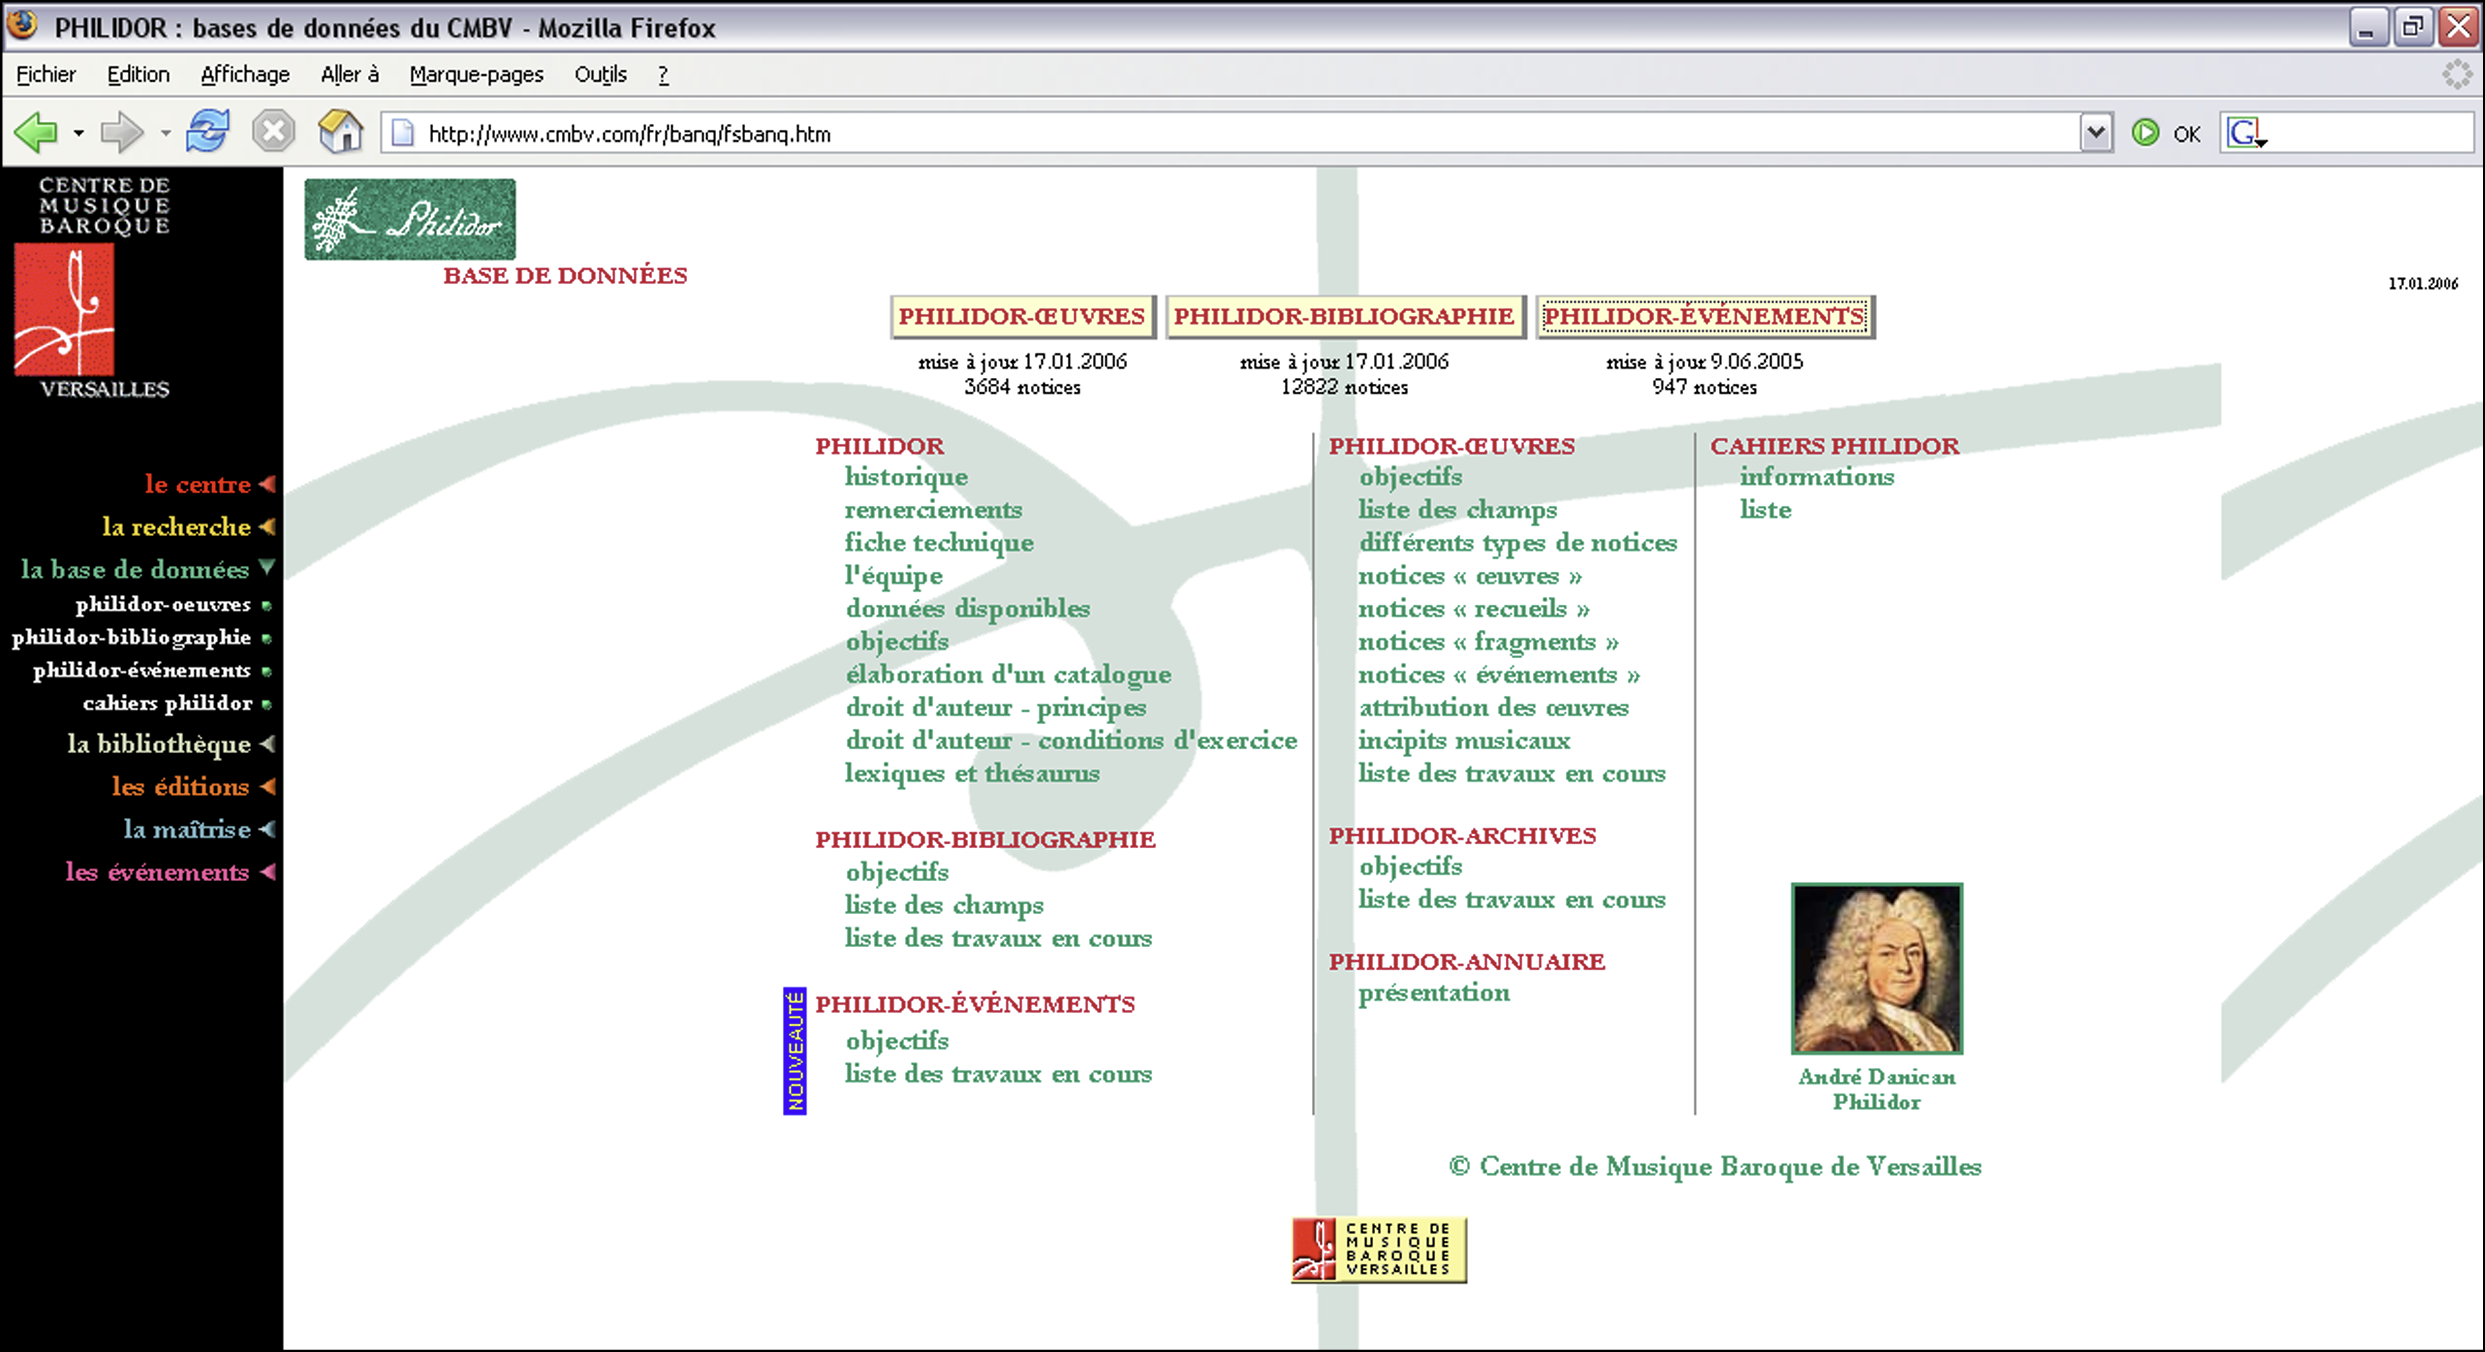
\includegraphics[width=\textwidth]{images/philidor1.png}
\end{figure}

La diffusion en ligne débuta avec le catalogue du petit motet imprimé, accompagné d'un texte de présentation et d'une introduction rédigés par Nathalie Berton, ainsi qu'un échantillon d'une vingtaine de fiches issues d'autres chantiers\footcite[Conseil scientifique, bilan de l'année 2001]{michelbenoitDocumentationTechniqueBibliographique1997}. Cette approche expérimentale permettait de tester les réactions des utilisateurs sur un corpus limité mais représentatif.

\subsubsection{Développement progressif des corpus et fonctionnalités}

L'intégration progressive des corpus prévoyait ensuite la poésie latine, des catalogues d'auteurs parmi lesquels on peut citer ceux de Sébastien Brossard, Jean Mignon, Claude-Mathieu Pellegrin et Henry Du Mont, ainsi que des recueils comme le manuscrit Deslauriers\footnote{F-Pn/ Rés Vma ms 571} et le recueil de motets et chansons de Tours\footnote{F-TO/ ms 168}.\footcite[Conseil scientifique, bilan de l'année 2001]{michelbenoitDocumentationTechniqueBibliographique1997}

L'interface est décrite comme \textquote{compliquée et sobre}, ainsi elle nécessitait une certaine familiarité avec l'outil\footcite[Rapport sur le projet Philidor de Jérémie Crublet, juin 2006]{michelbenoitDocumentationTechniqueBibliographique1997}. Cette complexité, héritée de l'usage interne initial, constituera un frein récurrent à l'appropriation par un public élargi.

\begin{figure}[h]
	\caption{Recherche dans l'index de \textit{Philidor I}} \label{philidor_i_index}
	\centering
	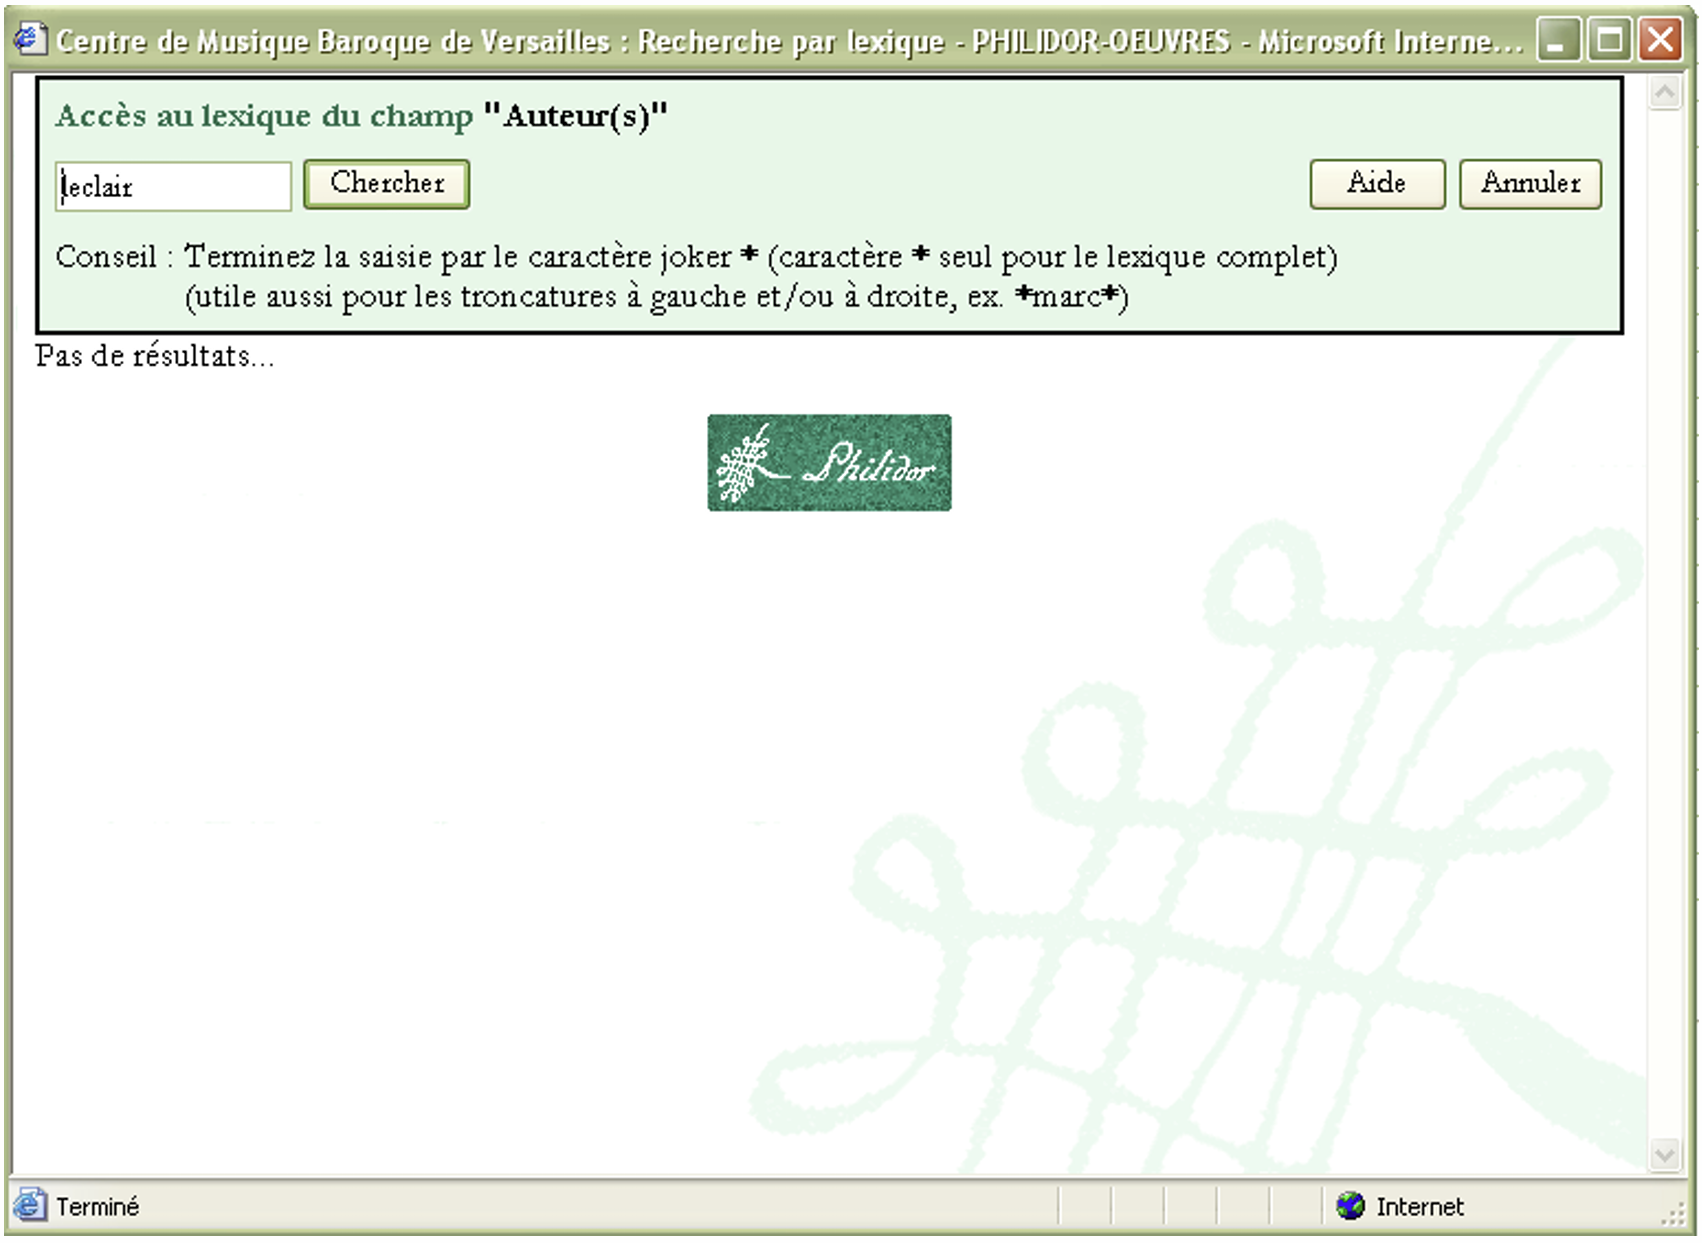
\includegraphics[width=\textwidth]{images/philidor1_index.png}
\end{figure}

D'autre part, l'enrichissement multimédia des fiches d'œuvres pouvaient se faire grâce à des images reproduisant la première page de la source principale. Cela facilitait la vérification visuelle des informations et le contrôle des \glspl{incipitmusical}\footcite[Conseil scientifique, bilan de l'année 2001]{michelbenoitDocumentationTechniqueBibliographique1997}. Ce processus de numérisation, retouche et intégration, débuté pour le petit motet imprimé, devait s'étendre aux œuvres de Brossard, Mignon, Pellegrin et Du Mont. Cette approche multimédia était innovante pour l'époque et préfigurait les développements ultérieurs.

Enfin, les documents dérivés et les formats de diffusion permettaient une amélioration de l'expérience utilisateur. La base proposait également des documents dérivés — bibliographies, tables d'incipits, dépouillements — disponibles au format Word, \gls{pdf} ou \gls{html}\footcite[Conseil scientifique, bilan de l'année 2001]{michelbenoitDocumentationTechniqueBibliographique1997}. Les fichiers PDF, destinés à protéger certains contenus, autorisaient l'impression mais limitaient la récupération informatique ; les fichiers \gls{html} étaient utilisés pour les documents libres, permettant leur consultation et leur réutilisation intégrale. Cette diversité des formats témoigne d'une réflexion aboutie sur les différents besoins des utilisateurs.

\subsubsection{Politique éditoriale et gestion des droits}

Enfin, la base diffusa également des travaux personnels de chercheurs, tels que l'inventaire de l'œuvre de Gossec, une table des œuvres de Marc-Antoine Charpentier et le catalogue de l'œuvre de Nicolas Clérambault\footcite[Conseil scientifique, bilan de l'année 2001]{michelbenoitDocumentationTechniqueBibliographique1997}.

Dès cette première phase, la base fut conçue pour accueillir et diffuser des travaux encore protégés par le droit d'auteur. Des contrats-types de promesse de cession de droits étaient établis, garantissant la confidentialité et la protection des données des chercheurs avant toute cession définitive. Ces dispositions avaient pour but d'encourager la contribution de travaux inédits sans craindre une exploitation prématurée ou non contrôlée\footcite[Conseil scientifique, bilan de l'année 2001]{michelbenoitDocumentationTechniqueBibliographique1997}. Cette préoccupation juridique révèle une approche professionnelle et raisonnée de la diffusion scientifique numérique.

\subsection{La migration sous JLB-NET : \textit{Philidor II}}

En 2006, la base entra dans sa deuxième phase, \textit{Philidor II}, avec l'adoption du logiciel JLB-NET, version adaptée de JLB-DOC pour une consultation en ligne\footcite[Rapport sur le projet Philidor de Jérémie Crublet, juin 2006]{michelbenoitDocumentationTechniqueBibliographique1997}. Cette migration témoigne de la volonté d'adapter l'outil aux exigences croissantes du web, tout en conservant la richesse fonctionnelle de la version précédente.

\subsubsection{Élargissement du périmètre et nouvelle vision éditoriale}

Cette refonte s'accompagna d'une nouvelle interface (cf. figure \ref{philidor_ii}) et d'un élargissement considérable du contenu. Le portail intégra désormais non seulement les bases documentaires, mais aussi des publications éditoriales comme les \textit{Cahiers Philidor}, les bulletins du \glslink{cmbv}{Centre} et le \textit{Bulletin Charpentier}, permettant aux chercheurs associés au \gls{cmbv} de publier directement leurs travaux en ligne\footcite[Présentation de la base de données PHILIDOR en Octobre 2010]{michelbenoitDocumentationTechniqueBibliographique1997}.

\begin{figure}[h]
	\caption{Accueil de \textit{Philidor II}} \label{philidor_ii}
	\centering
	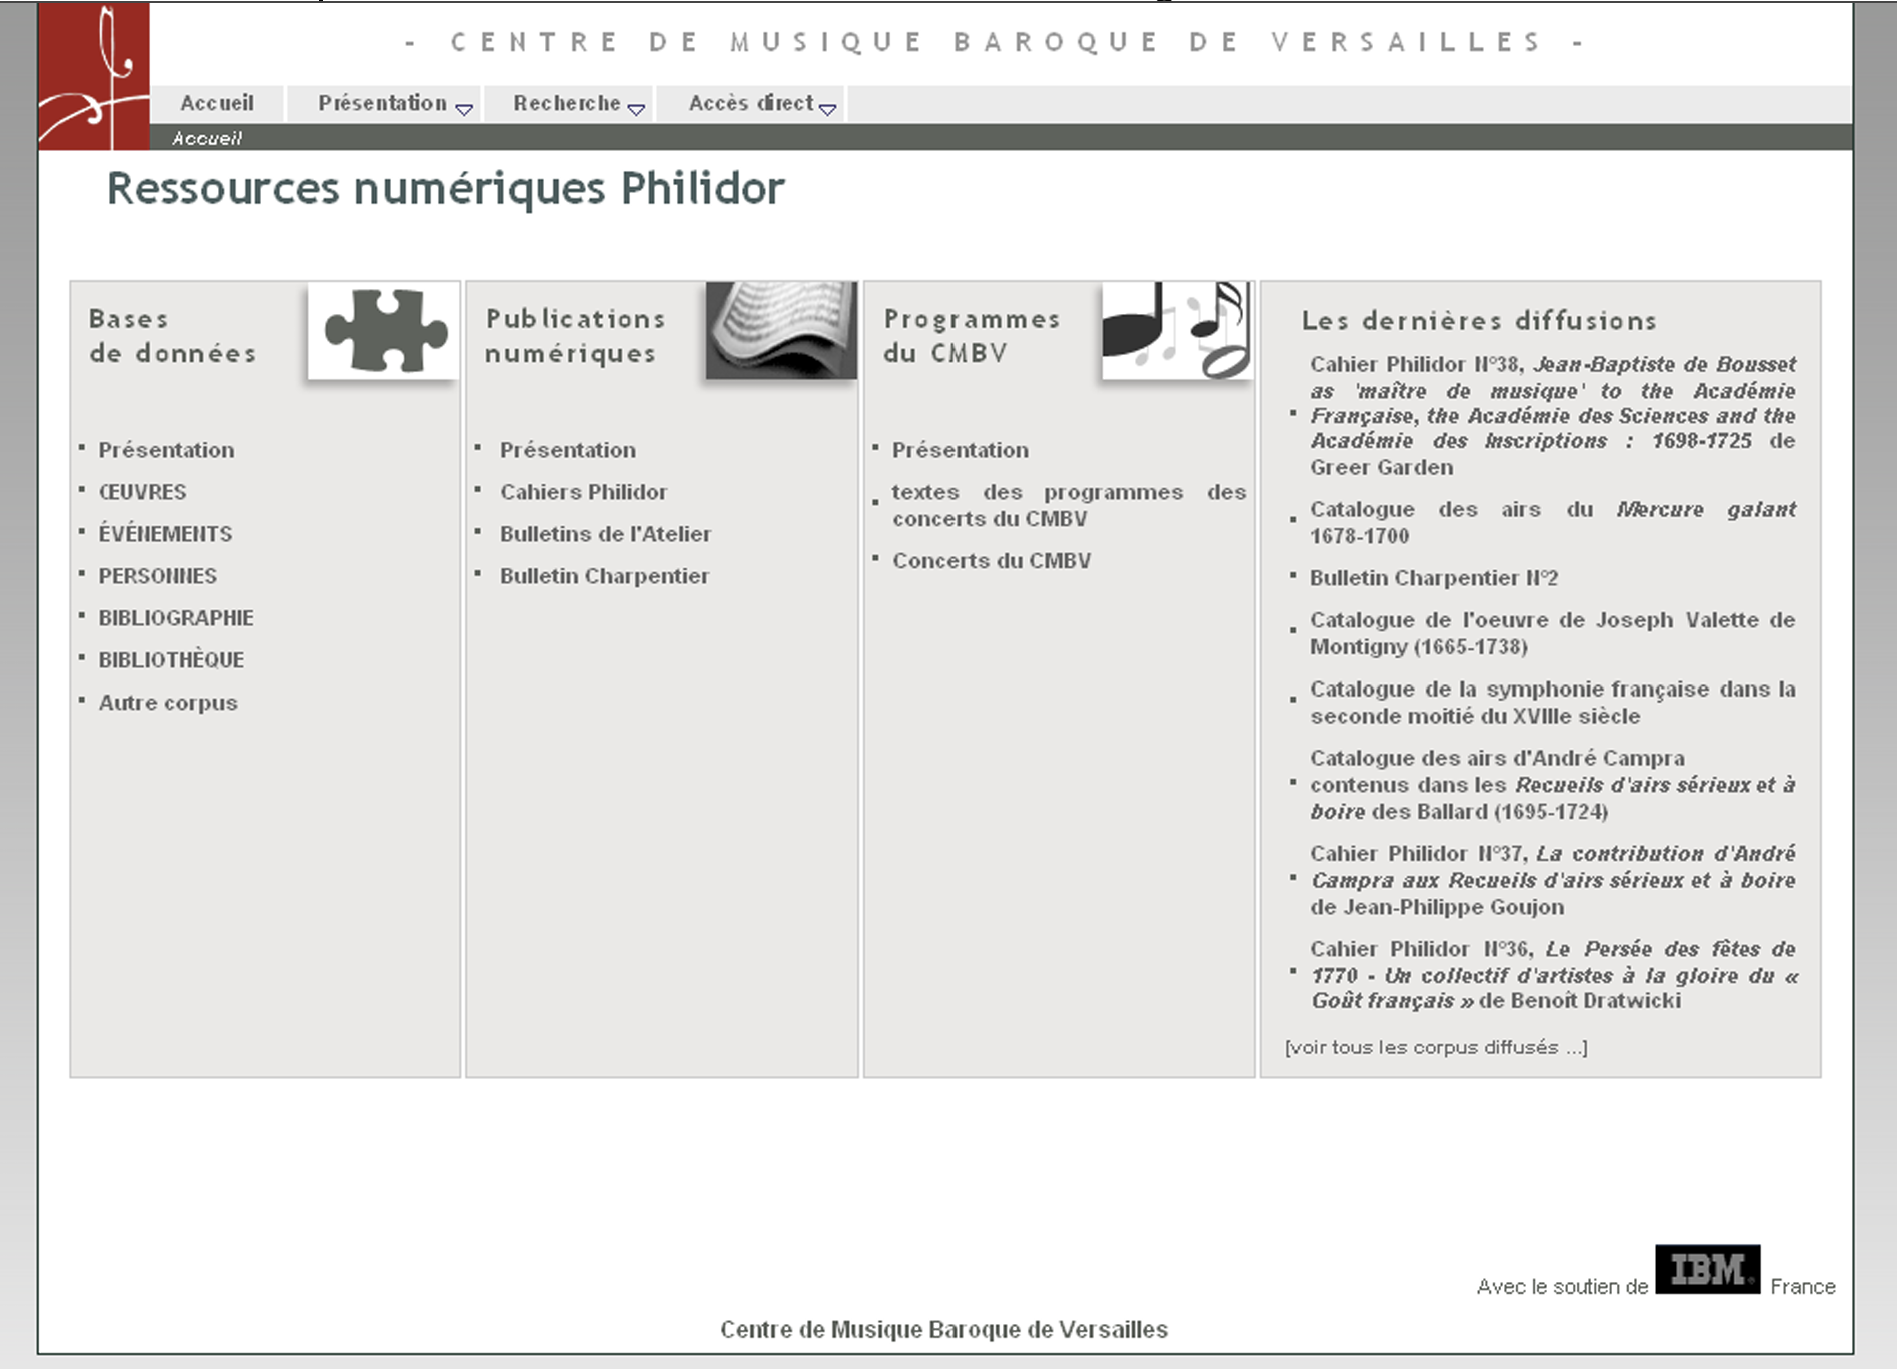
\includegraphics[width=\textwidth]{images/philidor2.png}
\end{figure}

L'objectif était de transformer \textit{Philidor} en un véritable portail de ressources dédié à la musique française des XVII\textsuperscript{e} et XVIII\textsuperscript{e} siècles, accessible aussi bien aux spécialistes qu'au grand public. Cette vision élargie marquait une évolution conceptuelle majeure : de base de données documentaire, \textit{Philidor} devenait une plateforme éditoriale complète.

\subsubsection{Limites techniques et ergonomiques identifiées}

Toutefois, malgré ces avancées, plusieurs limites apparurent rapidement. L'ergonomie, héritée d'un usage interne, s'avérait inadaptée à l'univers Internet : la navigation restait peu fluide, les liens entre notices étaient rares et le moteur de recherche manquait de puissance par rapport aux besoins exprimés\footcite[Présentation de la base de données PHILIDOR en Octobre 2010]{michelbenoitDocumentationTechniqueBibliographique1997}.

La plateforme ne facilitait pas le travail collaboratif et ne permettait pas la mise en commun dynamique des données existantes. De plus, la prise en main du logiciel JLB-NET était complexe pour les utilisateurs non formés, et les critiques des lecteurs sur l'ergonomie confirmaient que l'interface pouvait décourager la recherche prolongée\footcite[Présentation de la base de données PHILIDOR en Octobre 2010]{michelbenoitDocumentationTechniqueBibliographique1997}.

\subsubsection{Contraintes liées à la solution propriétaire}

Enfin, la dépendance à un logiciel propriétaire limitait les perspectives d'évolution\footcite[Rapport sur le projet Philidor de Jérémie Crublet, juin 2006]{michelbenoitDocumentationTechniqueBibliographique1997}. La création d'un nouveau portail de saisie reposant sur cette technologie n'était pas jugée souhaitable, car elle risquait de figer l'outil dans des contraintes techniques coûteuses à long terme. 

La nécessité de se mettre à niveau avec les standards et fonctionnalités du web 2.0 devint évidente afin de maintenir la pertinence de \textit{Philidor} face à l'abondance croissante d'informations disponibles en ligne\footcite[Présentation de la base de données PHILIDOR en Octobre 2010]{michelbenoitDocumentationTechniqueBibliographique1997}. Ce constat préparait la migration suivante vers des solutions plus ouvertes et flexibles.

\section[Diversification des outils]{Diversification des outils : panorama des solutions utilisées}

Face aux limites de la solution JLB et à l'évolution des besoins, le \gls{cmbv} s'engage, à partir de 2009, dans une politique de diversification de ses outils numériques. Cette stratégie répond à une double logique : d'une part, l'inadéquation croissante d'une solution unique face à la diversité des usages ; d'autre part, l'émergence de nouvelles technologies plus spécialisées et performantes dans leurs domaines respectifs.

Cette section examine cette période de transition, marquée par la migration de \textit{Philidor} vers \textit{eZ Publish} (\textit{Philidor III}) et l'émergence d'outils spécialisés pour différents usages. Elle analyse le développement des bases sous Omeka-S, solution open source qui permet une approche plus flexible de la gestion des collections numériques, et présente l'adoption du logiciel PMB pour la gestion de la bibliothèque. Cette diversification révèle une stratégie pragmatique d'adaptation aux besoins spécifiques de chaque type de contenu, mais soulève aussi des questions de cohérence et d'interopérabilité entre les différents systèmes.

\subsection{Migration vers \textit{eZ Publish} : \textit{Philidor III}}

\textit{Philidor III} marque une nouvelle étape dans l'histoire des bases de données du \gls{cmbv}, en adoptant une approche tournée vers une diffusion claire, continue et élargie des données sur Internet\footcite[Présentation de la base de données PHILIDOR en Octobre 2010]{michelbenoitDocumentationTechniqueBibliographique1997}. Sa mise en production démarre en 2009\footcite[Rapport sur le projet Philidor de Jérémie Crublet, juin 2006]{michelbenoitDocumentationTechniqueBibliographique1997}, marquant une rupture conceptuelle avec les approches précédentes.

\subsubsection{S'adapter aux nouveaux usages d'Internet}

Le passage de \textit{Philidor II} à \textit{Philidor III} a été motivé par les limites du logiciel JLB et par l’évolution rapide des usages d’Internet\footcite[La base de données Philidor - Bilan et enjeux de la nouvelle version, Jérémie Crublet et Michel Benoît, novembre 2010]{michelbenoitDocumentationTechniqueBibliographique1997}. Bien que performant pour créer des index et des \gls{thesaurus}, JLB s’avérait peu adapté à la diffusion en ligne : ergonomie lourde, navigation peu intuitive, référencement difficile et contraintes techniques freinant le travail collaboratif des chercheurs. Sa prise en main complexe et ses limites dans le partage de données rendaient son utilisation de plus en plus problématique\footcite{michelbenoitDocumentationTechniqueBibliographique1997}.  

Dans le même temps, les pratiques liées au Web 2.0 se généralisaient : en 2007, 95\,\% des recherches passaient par ce biais, alors que \textit{Philidor II} ne tirait pas parti de ces évolutions. Les internautes avaient besoin de recherches plein texte rapides et de données mieux reliées, tandis que les administrateurs devaient composer avec un système devenu obsolète et peu efficace pour gérer et diffuser l’information\footcite{michelbenoitDocumentationTechniqueBibliographique1997}.  

Face à ce constat, les objectifs de \textit{Philidor III} étaient d’accroître la visibilité de la base, d’adopter une architecture plus flexible et évolutive, d’intégrer de nouveaux types de documents (images, sons, etc.), et de mieux valoriser l’identité des contributeurs\footcite{michelbenoitDocumentationTechniqueBibliographique1997}. Il s’agissait aussi d’enrichir régulièrement le contenu, de renforcer les collaborations avec des institutions comme la \gls{bnf} et de donner à la base une dimension véritablement généraliste\footcite{michelbenoitDocumentationTechniqueBibliographique1997}.  

Cette évolution témoigne de l'adaptation du \gls{cmbv} aux pratiques numériques émergentes et à la demande croissante d'accès immédiat à l'information scientifique.

\subsubsection{Architecture technique, standards adoptés et strcture des données}

Sur le plan technique et financier, la solution a été l’abandon de JLB au profit de l'outil de gestion de contenu — en anglais, \gls{cms} — \textit{eZ Publish}. Un \gls{cms} permet de publier en ligne sans avoir à toucher le code \gls{html}\footnote{Langage informatique de base du web}. Ce dernier est saisi via un éditeur dans l'interface d'administration. Le \gls{cms} \textit{eZ Publish} intègre des fonctionnalités documentaires et est enrichi par un moteur de recherche libre \textit{Lucene}\footcite{michelbenoitDocumentationTechniqueBibliographique1997}. 

Cette nouvelle architecture basée sur des logiciels libres a permis de réduire considérablement les coûts, tout en offrant une meilleure intégration avec les usages du Web 2.0\footcite{michelbenoitDocumentationTechniqueBibliographique1997}. Elle a également simplifié la gestion des données et allégé le travail des contributeurs.

\textit{Philidor III} adopte également des standards documentaires largement reconnus tels que \textit{\gls{alto}}, \textit{\gls{ocr}}, \textit{Dublin Core} et \textit{\gls{tei}}\footcite[Présentation de la base de données PHILIDOR en Octobre 2010]{michelbenoitDocumentationTechniqueBibliographique1997}. Cette conformité aux standards internationaux marque une évolution vers une approche plus professionnelle et interopérable, facilitant les échanges avec d'autres institutions patrimoniales.

La structuration des données repose sur une approche \textquote{unitaire} : bien que celles-ci soient réparties en sous-ensembles (\textsc{Œuvres}, \textsc{Événements}, \textsc{Bibliographie}, \textsc{Biographies}), le système permet à chaque projet d'alimenter simultanément tous ces sous-ensembles. Les liens entre notices constituent un élément central, qu'ils soient actifs (créés à partir de la notice consultée) ou passifs (liens entrants depuis d'autres notices)\footcite[Rapport sur le projet Philidor de Jérémie Crublet, juin 2006]{michelbenoitDocumentationTechniqueBibliographique1997}.

Cette architecture relationnelle répond aux exigences de la recherche musicologique, où les informations s'organisent en réseaux complexes de relations entre œuvres, compositeurs, interprètes, lieux et événements. Concernant le contenu de la base, on peut citer les statistiques suivantes\footnote{Statistiques fin 2010 pour \textit{Philidor II}, en transition vers \textit{Philidor III}} :

\begin{itemize}
	\item 8 603 notices d'œuvres et recueils,
	\item 15 532 notices bibliographiques,
	\item 16 084 personnes indexées,
	\item 2 384 événements décrits,
	\item 25 corpus diffusés.
\end{itemize}

Ces chiffres témoignent de l'ampleur du travail accompli. Deux interfaces donnent accès à ces données, l'une consacrée à la base bibliographique et l'autre aux différents projets pouvant héberger tout type de notices.

\subsubsection{Interface utilisateur et stratégie de diffusion}

L'interface publique a été repensée pour simplifier la consultation : un \textit{champ de recherche unique} permet désormais d'interroger l'ensemble de la base, sans que l'utilisateur ait à sélectionner une sous-base au préalable\footcite[Rapport sur le projet Philidor de Jérémie Crublet, juin 2006]{michelbenoitDocumentationTechniqueBibliographique1997}. Cette simplification répond aux critiques d'ergonomie formulées concernant les versions précédentes. Le moteur de recherche autorise désormais la recherche plein texte ainsi qu'une recherche avancée par différents index, avec des liens dynamiques facilitant la navigation interne et externe\footcite[Présentation de la base de données PHILIDOR en Octobre 2010]{michelbenoitDocumentationTechniqueBibliographique1997}.

De plus, les adresses des notices et documents bénéficient d'\gls{url} pérennes grâce à l'adoption des identifiants \gls{ark}\footcite[Rapport sur le projet Philidor de Jérémie Crublet, juin 2006]{michelbenoitDocumentationTechniqueBibliographique1997}, garantissant leur stabilité et leur visibilité. Cette préoccupation témoigne d'une véritable considération pour la pérennité des références.

Par ailleurs, la diffusion peut désormais se faire de manière continue, au fur et à mesure de la relecture des notices et en accord avec les chercheurs, sans attendre la finalisation complète d'un projet\footcite[Présentation de la base de données PHILIDOR en Octobre 2010]{michelbenoitDocumentationTechniqueBibliographique1997}. Cette approche permet une valorisation plus rapide des travaux de recherche et une meilleure réactivité aux besoins des utilisateurs.

\subsubsection{Travail collaboratif et gestion des droits}

Contrairement aux versions précédentes, le dispositif favorise également le travail collaboratif. Les chercheurs peuvent suivre l'avancement des travaux des autres contributeurs et partager des index communs afin d'éviter les doublons et de mieux définir les axes de recherche\footcite[Rapport sur le projet Philidor de Jérémie Crublet, juin 2006]{michelbenoitDocumentationTechniqueBibliographique1997}. Cette dimension collaborative témoigne de l'évolution des pratiques scientifiques vers plus de transparence et de mutualisation.

La gestion des droits d'auteur est améliorée grâce à des informations précises sur les auteurs, les dates de diffusion et de modification, et le copyright ; des contrats-types de cession de droits ont été instaurés\footcite[Présentation de la base de données PHILIDOR en Octobre 2010]{michelbenoitDocumentationTechniqueBibliographique1997}. Le système permet aussi de travailler sur des données confidentielles tout en maintenant la rigueur scientifique grâce à une relecture préalable à la mise en ligne. 

Chaque contributeur conserve la maîtrise de la diffusion de ses notices, dispose d'un tableau de bord pour suivre ses modifications, accéder à ses brouillons et revenir à des versions antérieures\footcite[Présentation de la base de données PHILIDOR en Octobre 2010]{michelbenoitDocumentationTechniqueBibliographique1997}. Cette granularité dans la gestion des droits et des versions constitue une avancée significative par rapport aux systèmes précédents.

Ce sont donc 53 contributeurs en France et à l'étranger qui collaborent sur les différents projets. La diversité des contributeurs illustre le succès de la stratégie collaborative adoptée par le \gls{cmbv}.

En résumé, \textit{Philidor III} a marqué une étape stratégique et technique pour moderniser la base, la rendre plus accessible et collaborative, et mieux répondre aux exigences de la recherche contemporaine. Si \textit{Philidor II} ressemblait encore à une bibliothèque avec un catalogue papier, \textit{Philidor III} s’apparente désormais à une bibliothèque numérique interactive, proche d’un moteur de recherche, où l’information est plus riche, plus variée et plus facilement exploitable.

\subsection{Les bases sous Omeka-S}

Plusieurs bases de données du \gls{cmbv} sont construites et diffusées à l'aide de la plateforme Omeka-S. Cet outil, spécifiquement adapté à la gestion et à la valorisation des données patrimoniales, a permis d'unifier la présentation et la diffusion de corpus très divers, tout en garantissant leur structuration selon les standards du web de données.

\subsubsection{Une plateforme pour centraliser et valoriser les ressources}

Omeka-S joue un rôle de dépôt scientifique et éditorial au sein du \gls{cmbv}. L'interface de consultation, conçue pour favoriser l'exploration des métadonnées, s'appuie sur les standards du \gls{web-semantique} et offre des fonctionnalités avancées de recherche et de filtrage. En l'état actuel, l'instance d'Omeka-S du \gls{cmbv} n'exploite pas toutes les possibilités offertes par le \gls{web-semantique}. Cependant, il s'agit d'un objectif certain pour l'avenir du \glslink{cmbv}{Centre de Musique Baroque de Versailles}.

La base Fossard est la première base mise en ligne avec cet outil en décembre 2022. Elle a pour objectif initial de centraliser l'ensemble des ressources numériques produites ou collectées par le \gls{cmbv} dans le cadre de ses activités scientifiques. Elle permet de rassembler et de mettre en valeur des archives numériques, des périodiques numérisés, des introductions d'éditions critiques, des bases de données thématiques (compositeurs, institutions, imprimeurs), ainsi que des ressources iconographiques et audiovisuelles\footcite{FossardAnnuaireMusica2}. Les livres et articles numériques étaient déjà publiés en ligne depuis 2017. Depuis le lancement de la base sous Omeka-S, cette dernière est également alimentée en continu avec les \textit{Cahiers Philidor}, les archives scientifiques, et les préfaces des éditions critiques.

D'autres projets utilisent ou utiliseront prochainement cette infrastructure. La base AcadéC, en cours de réalisation, est associée au projet de recherche \textit{Les Académies de Concert en France (1710-1770)} et vise à recenser et rendre accessible toute la documentation sur les académies de musique actives entre 1710 et 1770. La collecte des données a débuté en février 2022 et la mise en ligne publique est prévue pour 2025\footcite{AcadeCAcademiesConcert}.

La base de données du projet \textit{Costumes de scène européens du XVIII\textsuperscript{e} siècle}\footnote{Page d'accueil de la base de données du projet \textit{Costumes de scène européens du XVIII\textsuperscript{e} siècle}, \url{https://omeka.cmbv.fr/s/costumes/page/accueil}}, finalisée par Petra, est ouverte au public et pourra être enrichie avec des costumes issus d'autres productions, en interconnexion avec la base de données du projet \textit{Du livret à la scène : l'Académie royale de musique de ses origines à Rameau}\footnote{Page d'accueil de la base de données du projet \textit{Du livret à la scène : l'Académie royale de musique de ses origines à Rameau}, \url{https://omeka.cmbv.fr/s/arm/page/accueil}}.

Enfin, la base de données du projet \textit{Les recueils Tours-168 et Deslauriers}\footnote{Page d'accueil de la base de données du projet \textit{Les recueils Tours-168 et Deslauriers}, \url{https://omeka.cmbv.fr/s/les-recueils-Tours-168-et-Deslauriers/page/accueil}}, récemment achevée, accompagne l'\gls{edition-numerique} du manuscrit musical n°168 de la Bibliothèque municipale de Tours, projet dirigé par Jean Duron. Elle a déjà intégré, en 2023, la mise à jour des premières pièces des manuscrits Deslauriers.

\subsubsection{Structure modulaire et interopérabilité}

Omeka-S est pensé pour la valorisation publique des données patrimoniales\footcite{BaseFossard}. Depuis une même installation, il est possible d'héberger plusieurs sites distincts, ce qui permet au \gls{cmbv} de mutualiser ses ressources et de faire évoluer son offre au gré des projets. Cette architecture modulaire répond parfaitement aux besoins d'une institution qui gère simultanément de multiples projets de recherche avec des temporalités et des publics différents.

Cette architecture modulaire repose sur les standards du \gls{web-semantique} et utilise les vocabulaires \gls{rdf}, avec une publication en \gls{jsonld}\footcite{OmekaProject}. Cela garantit une interopérabilité optimale avec d'autres bases et systèmes, et facilite l'intégration à des portails de diffusion plus larges. Cette approche technique permet au \gls{cmbv} de s'inscrire dans l'écosystème international des données liées (Linked Data).

Les modèles de ressources personnalisables\footcite{ResourceTemplatesOmeka} permettent, quant à eux, de structurer et d'homogénéiser la saisie et l'exploitation des métadonnées en fonction des besoins scientifiques ou éditoriaux propres à chaque projet. Cette flexibilité constitue un atout majeur pour une institution qui traite des corpus très hétérogènes, des partitions manuscrites aux enregistrements audiovisuels.

Par ailleurs, un riche écosystème de modules permet d'importer des données depuis des fichiers  au format \gls{csv}, Zotero ou d'autres bases\footcite{OmekaItemImporter}, ainsi que de proposer des visualisations interactives (cartographies, graphes, chronologies)\footcite{OmekaDataVisualization} facilitant la compréhension et l'exploration de corpus complexes. Ces outils de visualisation s'avèrent particulièrement utiles pour révéler des patterns dans les données musicologiques, comme l'évolution géographique des pratiques musicales ou les réseaux de relations entre compositeurs.

Omeka-S prend également en charge la gestion simultanée de documents texte, d'images, de partitions, d'enregistrements sonores, de vidéos et d'autorités (personnes, lieux, œuvres), ce qui correspond parfaitement à la diversité des collections du \gls{cmbv}.

\subsubsection{Pérennité, ouverture et évolutivité}

Logiciel open source, Omeka-S bénéficie du soutien d'une vaste communauté internationale d'utilisateurs et de développeurs. Sa pérennité est ainsi assurée par un suivi technique régulier et une capacité d'évolution rapide. Cette dimension communautaire constitue un gage de stabilité et d'innovation continue, particulièrement important pour des projets scientifiques à long terme.

L'API REST\footcite{RESTAPIOmeka} permet d'envisager des extensions fonctionnelles, des synchronisations automatiques ou des flux de travail collaboratifs, ainsi que l'ouverture future des données dans une logique FAIR\footnote{Facile à trouver, Accessible, Interopérable, Réutilisable}. Cette ouverture technique facilite l'intégration avec d'autres systèmes d'information et prépare l'évolution vers des pratiques de recherche plus collaboratives et transparentes.

Pour le \gls{cmbv}, l'adoption d'Omeka-S signifie la possibilité de mutualiser, structurer, valoriser et faire évoluer la diffusion des données scientifiques et patrimoniales, tout en assurant leur interopérabilité avec d'autres institutions culturelles ou de recherche. Cette stratégie s'inscrit dans une logique d'écosystème, où chaque outil spécialisé contribue à un ensemble cohérent et interopérable.

\subsection{Le catalogue de la bibliothèque sous le logiciel PMB}

PMB est une abréviation qui signifie PhpMyBibli. Il s'agit d'un \gls{sigb} développé en continu par l'entreprise française PMB Services depuis 2003. Il se distingue par sa capacité à répondre aux besoins spécifiques des bibliothèques de toutes tailles et typologies, notamment les bibliothèques spécialisées comme le \glslink{cmbv}{Centre de Musique Baroque de Versailles}.

\subsubsection{Les collections du \gls{cmbv} : diversité et spécialisation}

Avant de présenter plus en détails ce qu'est le logiciel, il convient d'avoir une vision d'ensemble des ressources de la bibliothèque du \gls{cmbv}. Cette dernière est une bibliothèque spécialisée de 25~000 documents incluant livres, partitions et documents audio-vidéo sur la musique française des XVII\textsuperscript{e} et XVIII\textsuperscript{e} siècles. Ces documents sont répartis entre 20~000 documents physiques et près de 4~000~Go d'objets numériques.

\paragraph{Le fonds documentaire} est composé des 6 000 volumes de livres et des 75 titres de périodiques qui offrent un panorama complet des études musicologiques et interdisciplinaires, allant des biographies de compositeurs aux travaux sur l’histoire, la danse, le théâtre ou encore la liturgie.\footcite{CentreMusiqueBaroqueb}. Cette diversité thématique reflète l'approche pluridisciplinaire adoptée par le \gls{cmbv} dans ses recherches sur la période baroque. À cela s'ajoute le fonds libraire de Marcelle Benoît, une musicologue et historienne de la musique spécialisée sur la musique française des XVII\textsuperscript{e} et XVIII\textsuperscript{e} siècles.

\paragraph{Les collections musicales} sont particulièrement riches, permettant une large sélection de morceaux pour le travail des Chantres. La bibliothèque comptent approximativement 12 000 volumes contenant des partitions, dont 1 500 volumes d'éditions monumentales\footcite{CentreMusiqueBaroqueb}. À ces partitions, s'ajoutent les plus de 600 titres présents en exemplaires multiples dans le fonds de la Maîtrise\footcite{CentreMusiqueBaroqueb}, témoignant de l'activité pédagogique et artistique du Centre.

\paragraph{Les fonds d'archives} conservés à la bibliothèque préservent la mémoire historique du \gls{cmbv}. On peut tout particulièrement citer le fonds d'archives de Jean Lionnet\footnote{Ce fonds concerne la musique romaine des XVII\textsuperscript{e}-XVIII\textsuperscript{e} siècles}, qui fut chercheur au \gls{cmbv} durant plusieurs années.

\paragraph{Les ressources audiovisuelles} comptent plus de 2 000 CD et quelques DVD qui permettent d'écouter ou regarder les captations audio ou vidéo des événements produits par le \gls{cmbv}. Ces ressources audiovisuelles constituent un témoignage précieux de l'activité artistique du \glslink{cmbv}{Centre} et de l'évolution des pratiques d'interprétation historiquement informée.

\subsubsection{Un logiciel open source : choix stratégique et avantages}

PMB est un \gls{sigb} libre et open source sous licence CeCILL. Il existe trois modes de commercialisation pour ce type de logiciel : les logiciels open source, les logiciels en abonnement et les logiciels avec cession de droit d'utilisation\footcite{maisonneuveLogicielsPourBibliotheques2021}. Parmi ces solutions, en 2023, les bibliothèques de lecture publique choisissent dans 28~\% des cas l'open source, contre 21~\% pour les bibliothèques spécialisées et 12~\% pour les bibliothèques universitaires\footcite{asselinLogicielsPourBibliotheques2024}.

Cette nature open source permet une transparence du code source, facilitant l'évolution du logiciel et son interopérabilité\footcite{jullienLogicielLibreGerer2022}. Pour une institution comme le \gls{cmbv}, cette approche offre une maîtrise technique et une indépendance par rapport aux éditeurs propriétaires, tout en bénéficiant d'une communauté active de développement.

PMB Services est le principal éditeur de PMB. Il développe la plupart des améliorations avant de les reverser dans le libre, garantissant que le logiciel reste à jour avec les évolutions du métier\footcite{PlaquettePMBServices}. C'est vers lui que le \gls{cmbv} s'est tourné pour déployer son instance de PMB. Cette solution permet au \gls{cmbv} d'avoir un accompagnement personnalisé quelle que soit l'aisance en informatique de ses équipes\footcite{PlaquettePMBServices}.

Les solutions open source sont considérées pour certains comme plus efficaces en raison de l'ouverture du code qui facilite la prise en compte des retours utilisateurs et des corrections de bugs\footcite{jullienLogicielLibreGerer2022}. De plus, elles ont un coût total de possession plus faible grâce à l'absence de frais de licence et à un meilleur respect des standards pour l'interopérabilité\footcite{jullienLogicielLibreGerer2022}.

\subsubsection{Architecture et fonctionnalités principales}

PMB s'articule autour de deux modules principaux : le module de gestion destiné aux professionnels et le module portail (OPAC) pour les usagers. Le module de gestion propose des fonctions spécialisées pour les bibliothécaires : circulation (prêt/retour), catalogage, gestion des autorités, éditions, diffusion sélective de l'information, acquisitions, \gls{cms} et administration.

\paragraph{La conformité aux normes internationales} est un aspect important du logiciel. Ce dernier respecte les normes \glslink{bibliotheconomie}{bibliothéconomiques} internationales : format \gls{unimarc} pour le catalogage, protocole Z39.50 pour l'import de notices bibliographiques, format d'échange ISO 2709 et \gls{xml}\footcite{marcolocascioMigrationBaseDonnees2024}. Cette conformité garantit l'interopérabilité avec les grands catalogues nationaux et internationaux.

\paragraph{Le modèle \glslink{frbr}{FRBR} et la structuration des données} offre un cadre d'autant plus normé pour la saisie et l'exploitation des données. En effet, le PMB intègre le modèle \gls{frbr}\footcite{PlaquettePMB}, que l'on peut traduire par spécifications fonctionnelles des notices bibliographiques, permettant une description fine des \textquote{entités}\footnote{On entend ici les œuvres, expressions, manifestations, items, personnes, lieux, événements} présents dans le catalogue. La \textquote{\gls{frbr}isation} permet de structurer les données autour des entités plutôt que des documents physiques, rendant le catalogue plus logique et plus facilement utilisable par les utilisateurs\footcite{bermesVersCatalogueOriente2016}. Dans cette optique, le \gls{cmbv} s'inscrit dans une réflexion globale de \gls{frbr}isation de ses autorités et de modernisation de son interface publique (OPAC). Cela permettra de regrouper toutes les éditions d'une même œuvre et de lier les données avec d'autres ressources sur le web\footcite{marcolocascioMigrationBaseDonnees2024a}. Par ailleurs, PMB permet de créer des vues en graphe des entités liées, facilitant l'exploration et la compréhension des éléments catalogués, et dispose d'un module de catalogage \gls{frbr} en graphe pour les cas complexes\footcite{servicesApplyFRBRModel}.

\paragraph{Les spécificités musicales} sont prises en charge grâce à une gestion spécifique des partitions musicales et du matériel d'orchestre. Pour ce faire, PMB a développé un module de gestion des nomenclatures. Cela permet une description précise de chaque instrument et de son rôle dans une formation musicale, y compris les instruments non standards et les ateliers de percussion. Ces fonctionnalités sont cruciales pour la programmation des saisons musicales (permettant des recherches fines par combinaison d'instruments ou durée) et pour la programmation des musiciens par les orchestres. Des numérisations de chaque partition peuvent être ajoutées en item numérique\footcite{servicesGerezVosPartitions}. Cette spécialisation musicale fait de PMB un choix particulièrement pertinent pour une institution comme le \gls{cmbv}, dont les collections et les besoins sont spécifiquement orientés vers la musique ancienne.

\section{La base bibliographique quitte \textit{Philidor}…}

L'évolution récente des outils du \gls{cmbv} est marquée par une décision stratégique majeure : la séparation de la base bibliographique du corpus \textit{Philidor}. Cette décision, qui peut paraître paradoxale au regard de l'ambition unificatrice initiale du projet, témoigne en réalité d'une maturité nouvelle dans la compréhension des enjeux numériques institutionnels.

Cette section analyse les raisons de cette décision et ses implications pour l'écosystème numérique de l'institution. Elle examine d'abord les différentes solutions envisagées, puis, détaille les étapes concrètes de la migration vers PMB, en analysant les défis techniques rencontrés, notamment la fusion des listes de vocabulaire contrôlé développées séparément au fil des années. Cette séparation illustre l'évolution vers un écosystème d'outils spécialisés, mais questionne aussi l'unité conceptuelle qui présidait à la création de \textit{Philidor}.

\subsection{Les solutions envisagées pour la base bibliographique}

Une étude a été conduite afin d'évaluer les options possibles pour la migration de la base bibliographique \textsc{Biblio}\footcite{laurentguilloEtudeEvolutionBase2023}, dont l'infrastructure technique devenait obsolète. Cette obsolescence s'inscrit dans un contexte plus large de vieillissement de la plateforme \textit{eZ Publish} et de nécessaire modernisation de l'ensemble des outils numériques du \gls{cmbv}.

Trois scénarios principaux ont été analysés, chacun présentant des implications distinctes en termes de coût, de complexité et de pérennité.

\subsubsection{Scénario 1 : L'abandon pur et simple}

La première option consistait à mettre fin au projet \textsc{Biblio}, ce qui impliquait la suppression de l'\gls{url} d'accès et la purge des données dans \textit{eZ Publish} afin de libérer de l'espace serveur\footcite{laurentguilloEtudeEvolutionBase2023}. Une variante prévoyait l'archivage préalable des données au format \gls{xml}, avec un coût initial faible par rapport aux autres scénarios, mais rendant la consultation difficile et non destinée au public\footcite{laurentguilloEtudeEvolutionBase2023}.

Cette solution aurait également généré une légère économie en ressources humaines, mais au prix d'une perte significative de visibilité et d'\gls{accessibilite} des données bibliographiques accumulées depuis des années. L'abandon représentait certes l'option la moins coûteuse à court terme, mais impliquait une rupture dans la mission de service public de diffusion des connaissances assurée par le \gls{cmbv}.

\subsubsection{Scénario 2 : La migration vers Zotero}

Le second scénario proposait de transférer les données vers Zotero\footcite{laurentguilloEtudeEvolutionBase2023}, un outil largement utilisé dans le monde académique pour la gestion de références bibliographiques. Cette solution présentait l'avantage de s'appuyer sur un outil éprouvé et familier de la communauté scientifique.

La base, hébergée sur les serveurs de Zotero\footnote{Chez Amazon Web Services}, aurait été alimentée à distance par un administrateur du \gls{cmbv} et accessible publiquement via une \gls{url} dédiée. Ce système offrait des fonctions de recherche simples et avancées, bien que la recherche par champs \textquote{sujet} restât partiellement limitée. 

Le coût de mise en place se situait dans une gamme moyenne, accompagné d'un abonnement annuel et d'un investissement en temps non négligeable pour la reprise facultative des données\footcite{laurentguilloEtudeEvolutionBase2023}. Cette option présentait l'intérêt de la simplicité technique, mais au prix d'une dépendance à un service externe et d'une moindre intégration avec l'écosystème numérique du \gls{cmbv}.

\subsubsection{Scénario 3 : La migration vers PMB}

Le troisième scénario envisageait la création d'une base distincte sous PMB\footcite{laurentguilloEtudeEvolutionBase2023}, le logiciel de gestion de bibliothèque déjà utilisé par le \gls{cmbv}, en mode \gls{saas}. Cette base simplifiée, dépourvue de gestion des autorités et de suivi des documents physiques, aurait permis de transférer aisément des notices entre \textsc{Biblio} et le catalogue principal de la bibliothèque, réduisant ainsi le travail de saisie\footcite{laurentguilloEtudeEvolutionBase2023}.

Comme nous avons pu le voir, PMB est un logiciel libre et largement répandu. De plus, il est maintenu par une entreprise française, ce qui renforce son attractivité. Cette option implique un investissement initial plus élevé que les autres scénarios, mais offre en contrepartie une intégration technique optimale et une maîtrise complète des données\footcite{laurentguilloEtudeEvolutionBase2023}.

\subsubsection{La solution retenue : rationalisation et intégration}

À l'issue de l'étude, la migration de \textsc{Biblio} vers PMB a été validée. Ce choix répond principalement à une volonté de rationalisation des outils et d'amélioration de l'\gls{accessibilite}. L'intégration de la base bibliographique dans le catalogue de la bibliothèque permet de disposer d'un seul environnement de gestion, facilitant la consultation pour les usagers et offrant la possibilité de vérifier immédiatement la disponibilité physique des références.

Le recours à un logiciel déjà en place évite de rechercher de nouveaux prestataires et limite le nombre d'interlocuteurs techniques, tout en garantissant la continuité du service. Cette logique de mutualisation s'inscrit dans une approche pragmatique de la gestion des systèmes d'information, privilégiant la cohérence d'ensemble aux solutions ponctuelles.

Comme nous avons pu le voir, PMB est structuré selon le modèle \gls{frbr}, assurant ainsi la conformité aux standards internationaux et ouvre la voie à des interconnexions avec d'autres catalogues majeurs tels que ceux de la Bibliothèque nationale de France ou du \gls{sudoc}. Sa flexibilité et son caractère évolutif permettent d'adapter l'interface publique aux besoins spécifiques du \gls{cmbv}, et de gérer différents types de notices, qu'elles correspondent à des documents physiques ou à de simples références bibliographiques.

\subsection{Étapes de la migration de la base bibliographique vers PMB}

La migration de la base de données bibliographique \textsc{Biblio} du \gls{cmbv} vers le système \textsc{PMB}, déjà en usage pour le catalogue de la bibliothèque, s'inscrit dans la volonté de remplacer l'ancien système \textit{eZ Publish} devenu obsolète et de centraliser la gestion des ressources bibliographiques dans une plateforme unique, performante et accessible au public. 

Le projet est structuré en quatre phases successives, chacune répondant à des défis techniques et organisationnels spécifiques. Cette approche méthodologique témoigne de la complexité des migrations de données patrimoniales et de la nécessité d'une planification rigoureuse.

\subsubsection{Phase 1 : Exportation des données et traitement automatisé}

Cette étape consiste à extraire l'ensemble des données depuis \textit{eZ Publish}. L'opération est confiée à la société ACATUS, qui produit un fichier \gls{xml} structuré, chaque type d'information (titre, auteur, date, résumé, etc.) étant encapsulé dans une balise dédiée\footcite{marcolocascioMigrationBaseDonnees2024}.

\subsubsection{Phase 2 : Importation des données et segmentation}

L'importation est assurée par PMB Services, qui élabore un script à partir du tableau de correspondance établi lors de l'exportation\footcite{marcolocascioMigrationBaseDonnees2024a}. Les données sont insérées dans les champs adéquats de la base PMB, en respectant les normes bibliographiques en vigueur.

Une innovation notable réside dans le traitement des champs de texte libre par un modèle d'intelligence artificielle entraîné pour réorganiser automatiquement les contenus selon les champs normalisés attendus par PMB. Cette structuration automatisée facilite la correspondance avec le tableau utilisé pour l'importation et témoigne de l'intégration de technologies émergentes dans les processus de migration patrimoniale. Le modèle en question est notamment entrainé sur le corpus de données du \gls{cmbv}. En effet, lors d'une réunion avec PMB Services, ces derniers ont fait part de leur enthousiasme pour tester leur modèle sur les données du \gls{cmbv}.

Trois ensembles distincts sont donc constitués : notices non vérifiées, notices vérifiées, et notices saisies manuellement après 2011. Cette segmentation facilite les opérations de contrôle et de validation ultérieures, en permettant un traitement différencié selon le niveau de fiabilité des données. Cette approche graduée reflète l'histoire complexe de la base, où différentes générations de données coexistent avec des niveaux de qualité variables.

\subsubsection{Phase 3 : Vérification, nettoyage et harmonisation}

Cette phase englobe la relecture et la validation des notices, le nettoyage des données, la suppression des doublons et, pour certaines catégories, la saisie manuelle au format \gls{unimarc}. Des tests d'affichage et de publication sont réalisés afin de vérifier la conformité et la lisibilité des notices.

Un travail est également mené sur l'interface publique pour envisager sa refonte, en tenant compte des spécificités des publics du \gls{cmbv} et des pratiques de recherche en musicologie. Cette réflexion sur l'interface illustre l'évolution des préoccupations : au-delà de la simple migration technique, il s'agit de repenser l'expérience utilisateur dans son ensemble.

Les glossaires et \glspl{thesaurus} existants sont fusionnés en un \gls{thesaurus} général conforme au standard \gls{skos}\footnote{voir sous-section \ref{fusion-theso} pour plus de détails sur cette problématique complexe}. Les fichiers \gls{pdf} actuellement hébergés sur \textit{eZ Publish} et accessibles au public sont transférés dans PMB, garantissant la continuité d'accès aux documents associés aux notices bibliographiques.

Cette dernière étape ne pouvait pas être automatisé par le prestataire. Pour répondre à cette difficulté technique, nous avons développé un script Python dédié permettant d’automatiser l’extraction et le téléchargement des fichiers \gls{pdf} encore hébergés sur l’ancienne plateforme (cf. annexe \ref{philidor_scrapper}). Ce programme navigue sur le catalogue en ligne, identifie pour chaque notice les documents associés, puis les renomme en normalisant le nom de fichier et les sauvegarde localement afin d’assurer leur réintégration ultérieure dans PMB. Le script intègre également des mécanismes de contrôle --- gestion des doublons, journalisation des opérations, sauvegardes intermédiaires --- afin de rendre le processus le plus fiable possible et de limiter les risques d’erreurs. Cet outil, conçu spécifiquement pour le \gls{cmbv} a permis de soulager les équipes techniques d’un travail manuel particulièrement chronophage.

\subsubsection{Phase 4 : Lancement et communication}

La dernière étape marque la désactivation définitive d'\textit{eZ Publish} et la mise en service officielle de la nouvelle base sous PMB\footcite{marcolocascioMigrationBaseDonnees2024a}. Cette transition technique s'accompagne d'une campagne d'information destinée à familiariser le public avec le nouvel outil et ses fonctionnalités.

Cette phase de communication révèle l'importance accordée à l'accompagnement des utilisateurs dans les transitions technologiques. Pour une institution patrimoniale, la continuité de service et l'acceptation par les publics constituent des enjeux aussi importants que la performance technique.

À plus long terme, cette migration s'inscrit dans une perspective d'harmonisation et de normalisation du catalogue PMB, avec l'intégration de standards internationaux comme la \gls{frbr}isation. L'architecture visée permettra de proposer deux modes de recherche : l'un pour les documents physiques de la bibliothèque, et l'autre pour un corpus bibliographique élargi intégrant toutes les références scientifiques disponibles.

\subsection{Le cas de la fusion des listes de vocabulaire contrôlé} \label{fusion-theso}

L'une des opérations les plus conséquentes lors de la migration fut la fusion des différentes listes de vocabulaire contrôlé développées au fil des années dans le catalogue de la bibliothèque et dans la base bibliographique. Cette problématique illustre parfaitement les défis posés par l'évolution des systèmes documentaires et la nécessité d'harmoniser des pratiques développées de manière autonome.

\subsubsection{Genèse de la fragmentation terminologique}

Au cours des décennies d'existence de \textit{Philidor} et de ses différentes évolutions, plusieurs \glspl{thesaurus} et listes de vocabulaire contrôlé se sont constitués de manière relativement indépendante. La base bibliographique \textsc{Biblio} avait développé ses propres termes d'indexation, adaptés aux spécificités de la littérature secondaire sur la musique baroque. En parallèle, le catalogue PMB de la bibliothèque avait établi son propre système de classification, davantage orienté vers la gestion des fonds matériels.  

Cette coexistence de deux systèmes terminologiques a progressivement entraîné une fragmentation conceptuelle entre les deux \glspl{thesaurus} : des termes similaires étaient exprimés différemment, certains concepts n’existaient que dans un des vocabulaires. Dans le cas d'une fusion, des doublons plus ou moins explicites pourraient compliquer la recherche documentaire. Cette situation reflète une tension récurrente dans les institutions documentaires, entre des besoins locaux, très pragmatiques, et l’exigence d’une interopérabilité plus large. 

\subsubsection{Pourquoi choisir SKOS ?}

\begin{quotation}
	\textquote{Dans certains cas, le choix d’un modèle de données est assez simple parce qu’il existe une adéquation complète entre l’objectif et une \glspl{ontologie} existante : par exemple, l’utilisation de \gls{skos} s’impose naturellement pour publier un \gls{thesaurus}.}\footcite{bermesCasPublierDonnees2013}
\end{quotation}

Le \gls{skos} est une recommandation du \gls{w3c}, conçue pour représenter sous forme de données structurées divers systèmes d’organisation des connaissances (\gls{thesaurus}, \glspl{taxonomie}, vocabulaires contrôlés, classifications). Basé sur les standards du Web sémantique (\gls{rdf}, \gls{owl}), il facilite la publication, l’échange et la réutilisation des vocabulaires via le Web.\footcite{SKOSSimpleKnowledge}

\gls{skos} fournit un modèle de données commun permettant d’identifier des concepts par des \gls{uri}, de leur attribuer des libellés préférentiels et alternatifs, et de décrire leurs relations hiérarchiques (\texttt{skos:broader} / \texttt{skos:narrower}) ainsi que des relations associatives ou de correspondance (ex. \texttt{skos:related}, \texttt{skos:exactMatch})\footcite{bermesCasPublierDonnees2013}. Il offre une voie de migration \textquote{légère} et peu coûteuse pour porter les vocabulaires existants vers un format Web sémantique. Grâce aux libellés alternatifs, il supporte les synonymes et facilite l’enrichissement des requêtes, tandis que ses relations hiérarchiques permettent d’explorer le vocabulaire par descentes ou montées structurelles.

\subsubsection{Préparation et normalisation des données}

La première étape de la fusion a consisté à préparer les données pour leur traitement automatique. Nous avons exporté les \glspl{thesaurus} issus du catalogue PMB au format \gls{skos}. Puis, nous les avons transformés en \gls{csv} grâce à une feuille \gls{xslt}\footnote{L’export \gls{skos} de PMB est relativement sommaire et nécessite un traitement intermédiaire (ici, une feuille \textsc{\gls{xslt}}) pour obtenir une structure exploitable.}. De son côté, la base bibliographique sur \textit{eZ Publish} a fourni son propre export. Ces différentes listes ont ensuite été fusionnées dans un fichier unique, compatible \gls{skos}.

Un important travail de nettoyage a suivi, mobilisant des outils tels qu’OpenRefine\footnote{OpenRefine est un logiciel libre couramment utilisé pour l’analyse et la correction de données tabulaires. Il permet notamment de détecter des doublons approximatifs grâce à des \glslink{algorithmie}{algorithmes} de similarité.} pour identifier et supprimer les doublons, d’abord via des filtres automatiques, puis par vérification manuelle. Cette étape fut complétée par un enrichissement sémantique, à l’aide de nombreux dictionnaires spécialisés\footnote{Escudier, Léon et Marie (1872). \textit{Dictionnaire de musique théorique et historique} (5\textsuperscript{e} éd.). E. Dentu ; Furetière, Antoine (1690, 1701). \textit{Dictionnaire universel} ; Bouissou, Sylvie (1996). \textit{Vocabulaire de la musique baroque}. Minerve ; Benoit, Marcelle (dir.) (1992). \textit{Dictionnaire de la musique en France aux XVII\textsuperscript{e} et XVIII\textsuperscript{e} siècles}. Fayard ; Rousseau, Jean-Jacques (1768). \textit{Dictionnaire de la musique}. Duchesne ; Académie française, \textit{Dictionnaire} (4\textsuperscript{e} et 9\textsuperscript{e} éd.) ; Le Robert ; Larousse ; Wright, Rowland (1941). \textit{Dictionnaire des instruments de musique}. Battley Brothers ; etc.}, qui ont permis d’ajouter des définitions et de préciser l’usage de certains termes par des notes d’application (\texttt{skos:scopeNote}).

\subsubsection{De la donnée brute à la hiérarchie SKOS}

Une fois les listes préparées et normalisées, un pipeline de traitement a été mis en place afin de construire automatiquement une hiérarchie exploitable (cf. annexe \ref{pipeline-hierarchisation-theso}). Celui-ci reposait sur une architecture modulaire, organisée en plusieurs phases successives :

\paragraph{Phase 1 - Traitement et préparation des données :}
Les données brutes sont transformées et normalisées, afin de créer des index lexicaux facilitant la détection ultérieure des relations hiérarchiques.

\paragraph{Phase 2 - Détection par motifs lexicaux :}  
Des règles linguistiques simples, comme l’inclusion de mots ou des constructions de type \textquote{X de Y}, permettent d’identifier des candidats à des relations de type \texttt{skos:broader}.

\paragraph{Phase 3 - Analyse de similarité lexicale :}  
Des métriques de proximité lexicale (sous-chaînes, coefficient de Jaccard, distances d’édition) servent à repérer des regroupements terminologiques et des familles morphologiques.

\paragraph{Phase 4 - Découverte sémantique contextuelle :}  
Une approche de traitement automatique du langage naturel, en anglais \gls{nlp}, enrichit la détection par des \textit{embeddings} sémantiques et une analyse de graphe, permettant de mettre en évidence de nouvelles relations hiérarchiques.

\paragraph{Phase 5 - Construction de la hiérarchie :}  
Les relations détectées sont agrégées et validées, avec gestion des poly-hiérarchies et réduction des redondances, pour obtenir un graphe cohérent permettant ensuite une validation manuelle via le terminal des parents candidats, c'est-à-dire des parents proposé par le script pour un groupe donné.

\paragraph{Phase 6 - Optimisation structurelle :}  
Un module final affine la hiérarchie en supprimant les cycles, réduisant les relations transitives superflues et limitant la complexité des poly-hiérarchies.

\paragraph{Phase 7 - Génération des fichiers de sortie :}  
Enfin, le \gls{thesaurus} hiérarchisé est exporté au format \gls{skos}, accompagné de statistiques de validation et de qualité.

\subsubsection{Un enjeu méthodologique et conceptuel}

La fusion des vocabulaires contrôlés ne se réduit pas à un exercice technique. Elle engage des choix épistémologiques sur la définition des concepts, leur granularité et leur organisation. Les doublons ne sont pas toujours triviaux à trancher : la question de savoir si deux termes renvoient au même concept ou à deux réalités distinctes relève souvent d’une expertise humaine.  

Le recours à une pipeline \glslink{algorithmie}{algorithmique} permet d’automatiser une grande partie du processus. Elle fait gagner du temps, mais ne dispense pas d’une validation experte. Cette validation garantit non seulement la cohérence terminologique, mais aussi la pertinence scientifique des regroupements opérés. L’harmonisation réalisée constitue ainsi un préalable indispensable à l’exploitation scientifique des données et à leur interopérabilité dans des environnements documentaires plus larges.


\section*{Conclusion du chapitre}

L'histoire des outils numériques du \gls{cmbv} révèle une trajectoire exemplaire de la transformation numérique des institutions patrimoniales. De la base de données locale des années 1990 à l'écosystème complexe d'aujourd'hui, chaque étape témoigne d'une adaptation constante aux évolutions technologiques et aux besoins croissants des utilisateurs.

Cette évolution s'organise autour de trois grandes périodes. La première, dominée par les solutions JLB, correspond à l'émergence de l'informatique documentaire et à la constitution des premiers corpus numériques. Elle se caractérise par une approche unifiée, incarnée par la vision initiale de \textit{Philidor} comme outil centralisateur de toutes les connaissances sur la musique baroque française.

La deuxième période, marquée par l'adoption d'\textit{eZ Publish} pour \textit{Philidor III}, illustre l'adaptation aux exigences du web et l'ouverture vers un public élargi. Cette phase révèle une professionnalisation des pratiques numériques et une meilleure compréhension des enjeux de diffusion en ligne.

La troisième période, encore en cours, se caractérise par la diversification des outils et la spécialisation des usages. L'adoption d'Omeka-S pour certains projets, le déploiement de PMB pour la bibliothèque et la séparation de la base bibliographique témoignent d'une approche plus pragmatique, privilégiant l'efficacité fonctionnelle à l'unité systémique.

Cette évolution soulève des questions fondamentales sur l'équilibre entre spécialisation et cohérence, entre innovation et pérennité, entre ouverture et contrôle. Les défis techniques rencontrés, notamment lors de la fusion des vocabulaires contrôlés, illustrent la complexité croissante des écosystèmes numériques patrimoniaux et la nécessité d'une approche systémique de leur gestion.

L'analyse de cette trajectoire éclaire les enjeux contemporains du numérique patrimonial et prépare la réflexion sur les perspectives d'évolution à venir, qui feront l'objet des chapitres suivants.